\documentclass[12pt,a4paper]{article}
\usepackage[utf8]{vietnam}
\usepackage{amsmath,amssymb,mathrsfs}
\usepackage{graphicx}
\usepackage{tikz}
\usepackage{array}
\usepackage[top=1.4cm,bottom=1.5cm,left=1.6cm,right=1.5cm]{geometry}
\usepackage{fancyhdr}
\usepackage{tcolorbox}
\tcbuselibrary{skins}
\usepackage[dethi]{ex_test}

\makeatletter
\@ifundefined{c@bt}{\newcounter{bt}}{}
\makeatother

\pagestyle{fancy}
\fancyhf{}
\renewcommand{\headrulewidth}{0pt}
\renewcommand{\footrulewidth}{0.4pt}
\lfoot{\footnotesize\textsl{Lớp Toán Cô Thúy -- SĐT: 0935.322.328 -- 50/2C Phạm Thị Liên}}
\rfoot{\footnotesize\textsl{Trang \thepage/4 -- Mã đề 0102}}

\begin{document}

% KHUNG TIÊU ĐỀ CHUẨN TỐI ƯU LỚP TOÁN CÔ THÚY
\noindent
\begin{tabular}{|p{6.6cm}|p{6.4cm}|>{\centering\arraybackslash}p{3.2cm}|}
\hline
\begin{minipage}{6.6cm}
\vspace{5pt}
\centering
{\large\bfseries\color{blue!80!black} LỚP TOÁN CÔ THÚY}\\[4pt]
\textbf{SĐT:} 0935.322.328\\[3pt]
\textbf{Địa chỉ:} 50/2C Phạm Thị Liên
\vspace{5pt}
\end{minipage}
&
\multicolumn{2}{p{10.0cm}|}{
\begin{minipage}{10.0cm}
\vspace{5pt}
\centering
{\bfseries\color{red!80!black} ĐỀ KHẢO SÁT CHẤT LƯỢNG TOÁN 12}\\[4pt]
\textbf{THPT Số 3 Bảo Thắng (2026 -- 2027)}\\[3pt]
\textit{Thời gian làm bài: 25 phút}
\vspace{5pt}
\end{minipage}
} \\
\hline
\rule{0pt}{15pt}Họ và tên: \dotfill\rule[-5pt]{0pt}{5pt} &
\rule{0pt}{15pt}Số báo danh: \dotfill\rule[-5pt]{0pt}{5pt} &
\rule{0pt}{15pt}\textbf{Mã đề 0102}\rule[-5pt]{0pt}{5pt} \\
\hline
\end{tabular}
\vspace{0.2cm}

\begin{flushleft}
	{\color{blue!50!green}\fbox{\fontfamily{qag}\bfseries\selectfont PHẦN I. Câu trắc nghiệm nhiều phương án lựa chọn}}
	\textit{\small (Thí sinh trả lời từ câu 1 đến câu 12. Mỗi câu hỏi thí sinh chỉ chọn một phương án.)}
\end{flushleft}
\setcounter{ex}{0}
\setcounter{bt}{0}

% Câu 1
\begin{ex}
	Cho hàm số $y = f(x)$ có bảng biến thiên như dưới đây:
	\begin{center}
	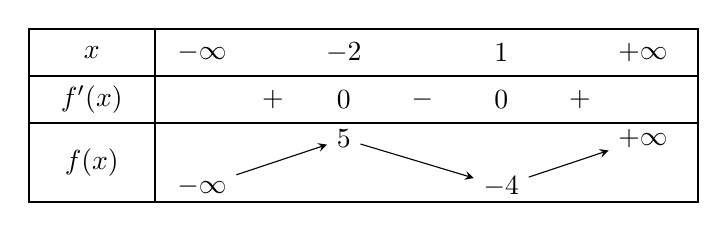
\begin{tikzpicture}[>=stealth,scale=1]
	  \draw[thick] (0,0) rectangle (8.5,-2.2);
	  \draw[thick] (0,-0.6) -- (8.5,-0.6);
	  \draw[thick] (0,-1.2) -- (8.5,-1.2);
	  \draw[thick] (1.6,0) -- (1.6,-2.2);
	  \node at (0.8,-0.3) {$x$};
	  \node at (0.8,-0.9) {$f'(x)$};
	  \node at (0.8,-1.7) {$f(x)$};
	  \node at (2.2,-0.3) {$-\infty$};
	  \node at (4.0,-0.3) {$-2$};
	  \node at (6.0,-0.3) {$1$};
	  \node at (7.8,-0.3) {$+\infty$};
	  \node at (3.1,-0.9) {$+$};
	  \node at (4.0,-0.9) {$0$};
	  \node at (5.0,-0.9) {$-$};
	  \node at (6.0,-0.9) {$0$};
	  \node at (7.0,-0.9) {$+$};
	  \node (p1) at (2.2,-2.0) {$-\infty$};
	  \node (p2) at (4.0,-1.4) {$5$};
	  \node (p3) at (6.0,-2.0) {$-4$};
	  \node (p4) at (7.8,-1.4) {$+\infty$};
	  \draw[->] (p1) -- (p2);
	  \draw[->] (p2) -- (p3);
	  \draw[->] (p3) -- (p4);
	\end{tikzpicture}
	\end{center}
	Khoảng nào sau đây là một khoảng đồng biến của hàm số?
	\choice
	{\True $(-\infty; -2)$}
	{$(-2; 1)$}
	{$(-2; +\infty)$}
	{$(-\infty; 1)$}
	\loigiai{}
\end{ex}

% Câu 2
\begin{ex}
	Cho hàm số $y = f(x)$ có đạo hàm $f'(x) = 3(x + 1)(x - 3)$ với mọi $x \in \mathbb{R}$. Điểm cực tiểu của hàm số đã cho là
	\choice
	{$x = -1$}
	{$x = 0$}
	{$x = 9$}
	{\True $x = 3$}
	\loigiai{}
\end{ex}

% Câu 3
\begin{ex}
	Cho hàm số $y = \dfrac{2x - 3}{x + 2}$. Đường tiệm cận đứng của đồ thị là
	\choice
	{$x = 2$}
	{\True $x = -2$}
	{$y = 2$}
	{$y = -2$}
	\loigiai{}
\end{ex}

% Câu 4
\begin{ex}
	Cho hàm số $y = \dfrac{3x + 1}{x - 2}$. Đường tiệm cận ngang của đồ thị là
	\choice
	{$y = -2$}
	{$x = 3$}
	{\True $y = 3$}
	{$y = 1$}
	\loigiai{}
\end{ex}

% Câu 5
\begin{ex}
	Cho hàm số $y = x - 1 + \dfrac{2}{x - 1}$. Phương trình đường tiệm cận xiên của đồ thị hàm số là
	\choice
	{$y = x + 1$}
	{$y = -x + 1$}
	{$x = 1$}
	{\True $y = x - 1$}
	\loigiai{}
\end{ex}

% Câu 6
\begin{ex}
	Đồ thị hàm số $y = 2 + \dfrac{4}{x - 1}$ có tâm đối xứng là
	\choice
	{\True $I(1; 2)$}
	{$I(2; 1)$}
	{$I(-1; 2)$}
	{$I(1; -2)$}
	\loigiai{}
\end{ex}

\newpage
% Câu 7
\begin{ex}
	Cho hàm số $y = f(x)$ có đạo hàm $f'(x) = (x + 2)(x - 1)^2(x - 3)$ với mọi $x \in \mathbb{R}$. Số điểm cực trị của hàm số là
	\choice
	{\True $2$}
	{$1$}
	{$3$}
	{$4$}
	\loigiai{}
\end{ex}

% Câu 8
\begin{ex}
	Cho hàm số $y = x + 2 - \dfrac{1}{x + 1}$. Giao điểm hai đường tiệm cận của đồ thị hàm số là
	\choice
	{$I(1; 3)$}
	{$I(-1; -2)$}
	{$I(1; -1)$}
	{\True $I(-1; 1)$}
	\loigiai{}
\end{ex}

% Câu 9
\begin{ex}
	Cho hàm số $y = f(x) = x^3 - 3x$. Khẳng định nào sau đây đúng?
	\choice
	{Hàm số có đúng một điểm cực trị}
	{\True Hàm số có cực đại tại $x = -1$ và cực tiểu tại $x = 1$}
	{Hàm số nghịch biến trên $(-\infty; -1)$}
	{Tâm đối xứng của đồ thị là $I(1; 0)$}
	\loigiai{}
\end{ex}

% Câu 10
\begin{ex}
	Cho hàm số phân thức $y = \dfrac{ax + b}{cx + d}$ ($ac \ne 0, ad - bc \ne 0$) có bảng biến thiên như dưới đây:
	\begin{center}
	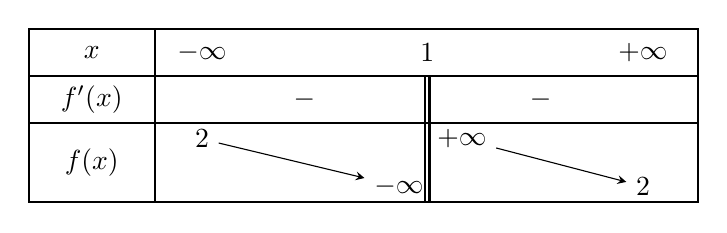
\begin{tikzpicture}[>=stealth,scale=1]
	  \draw[thick] (0,0) rectangle (8.5,-2.2);
	  \draw[thick] (0,-0.6) -- (8.5,-0.6);
	  \draw[thick] (0,-1.2) -- (8.5,-1.2);
	  \draw[thick] (1.6,0) -- (1.6,-2.2);
	  \draw[thick] (5.03,-0.6) -- (5.03,-2.2);
	  \draw[thick] (5.09,-0.6) -- (5.09,-2.2);
	  \node at (0.8,-0.3) {$x$};
	  \node at (0.8,-0.9) {$f'(x)$};
	  \node at (0.8,-1.7) {$f(x)$};
	  \node at (2.2,-0.3) {$-\infty$};
	  \node at (5.06,-0.3) {$1$};
	  \node at (7.8,-0.3) {$+\infty$};
	  \node at (3.5,-0.9) {$-$};
	  \node at (6.5,-0.9) {$-$};
	  \node (p1) at (2.2,-1.4) {$2$};
	  \node (p2) at (4.7,-2.0) {$-\infty$};
	  \node (p3) at (5.5,-1.4) {$+\infty$};
	  \node (p4) at (7.8,-2.0) {$2$};
	  \draw[->] (p1) -- (p2);
	  \draw[->] (p3) -- (p4);
	\end{tikzpicture}
	\end{center}
	Hàm số nào dưới đây có bảng biến thiên đã cho?
	\choice
	{$y = \dfrac{2x - 5}{x - 1}$}
	{$y = \dfrac{x + 1}{x - 1}$}
	{\True $y = \dfrac{2x + 1}{x - 1}$}
	{$y = \dfrac{2x + 1}{x + 1}$}
	\loigiai{}
\end{ex}

% Câu 11
\begin{ex}
	\immini{
		Cho hàm số bậc ba $y = f(x)$ có đồ thị như hình bên. Hàm số nào dưới đây có đồ thị như hình đã cho?
		\choice
		{$y = -x^3 + 3x$}
		{\True $y = x^3 - 3x$}
		{$y = x^3 + 3x$}
		{$y = x^3 - 3x + 1$}
	}{
		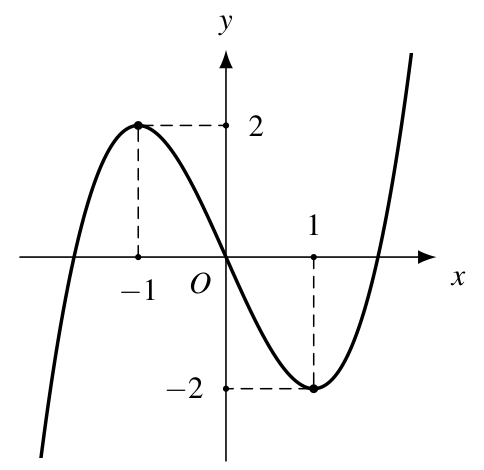
\includegraphics[width=4.5cm]{c11_hinh.png}
	}
	\loigiai{}
\end{ex}

% Câu 12
\begin{ex}
	Cho hàm số $y = f(x)$ có bảng biến thiên như dưới đây:
	\begin{center}
	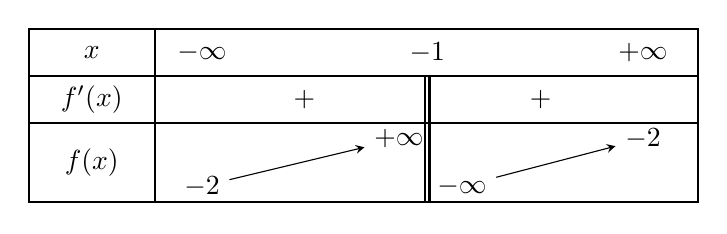
\begin{tikzpicture}[>=stealth,scale=1]
	  \draw[thick] (0,0) rectangle (8.5,-2.2);
	  \draw[thick] (0,-0.6) -- (8.5,-0.6);
	  \draw[thick] (0,-1.2) -- (8.5,-1.2);
	  \draw[thick] (1.6,0) -- (1.6,-2.2);
	  \draw[thick] (5.03,-0.6) -- (5.03,-2.2);
	  \draw[thick] (5.09,-0.6) -- (5.09,-2.2);
	  \node at (0.8,-0.3) {$x$};
	  \node at (0.8,-0.9) {$f'(x)$};
	  \node at (0.8,-1.7) {$f(x)$};
	  \node at (2.2,-0.3) {$-\infty$};
	  \node at (5.06,-0.3) {$-1$};
	  \node at (7.8,-0.3) {$+\infty$};
	  \node at (3.5,-0.9) {$+$};
	  \node at (6.5,-0.9) {$+$};
	  \node (p1) at (2.2,-2.0) {$-2$};
	  \node (p2) at (4.7,-1.4) {$+\infty$};
	  \node (p3) at (5.5,-2.0) {$-\infty$};
	  \node (p4) at (7.8,-1.4) {$-2$};
	  \draw[->] (p1) -- (p2);
	  \draw[->] (p3) -- (p4);
	\end{tikzpicture}
	\end{center}
	Khẳng định nào sau đây đúng?
	\choice
	{Hàm số nghịch biến trên $(-\infty; -1)$}
	{Hàm số có cực trị tại $x = -1$}
	{\True Hàm số đồng biến trên từng khoảng $(-\infty; -1)$ và $(-1; +\infty)$}
	{Đồ thị không có tiệm cận ngang}
	\loigiai{}
\end{ex}

\newpage
\begin{flushleft}
	{\color{blue!50!green}\fbox{\fontfamily{qag}\bfseries\selectfont PHẦN II. Câu trắc nghiệm đúng sai}}
	\textit{\small (Thí sinh trả lời từ câu 1 đến câu 4. Trong mỗi ý a), b), c), d) ở mỗi câu, thí sinh chọn đúng hoặc sai.)}
\end{flushleft}
\setcounter{ex}{0}
\setcounter{bt}{0}

% Phần II Câu 1
\begin{ex}
	Cho hàm số $y = f(x) = x^3 - 3x^2 + 2$. Xét tính đúng, sai của các phát biểu sau:
	\choiceTF
	{\True Đạo hàm của hàm số là $f'(x) = 3x(x - 2)$}
	{\True Hàm số nghịch biến trên khoảng $(0; 2)$}
	{Hàm số đạt cực đại tại $x = 2$}
	{\True Bảng biến thiên dưới đây là bảng biến thiên của hàm số đã cho
		\begin{center}
		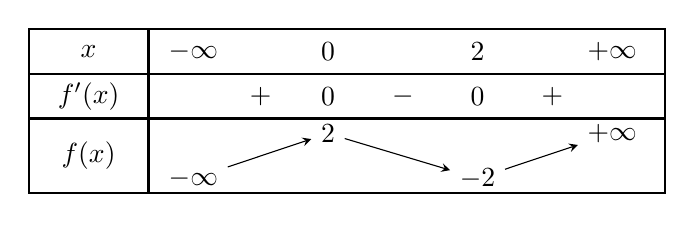
\begin{tikzpicture}[>=stealth,scale=0.95]
		  \draw[thick] (0,0) rectangle (8.5,-2.2);
		  \draw[thick] (0,-0.6) -- (8.5,-0.6);
		  \draw[thick] (0,-1.2) -- (8.5,-1.2);
		  \draw[thick] (1.6,0) -- (1.6,-2.2);
		  \node at (0.8,-0.3) {$x$};
		  \node at (0.8,-0.9) {$f'(x)$};
		  \node at (0.8,-1.7) {$f(x)$};
		  \node at (2.2,-0.3) {$-\infty$};
		  \node at (4.0,-0.3) {$0$};
		  \node at (6.0,-0.3) {$2$};
		  \node at (7.8,-0.3) {$+\infty$};
		  \node at (3.1,-0.9) {$+$};
		  \node at (4.0,-0.9) {$0$};
		  \node at (5.0,-0.9) {$-$};
		  \node at (6.0,-0.9) {$0$};
		  \node at (7.0,-0.9) {$+$};
		  \node (p1) at (2.2,-2.0) {$-\infty$};
		  \node (p2) at (4.0,-1.4) {$2$};
		  \node (p3) at (6.0,-2.0) {$-2$};
		  \node (p4) at (7.8,-1.4) {$+\infty$};
		  \draw[->] (p1) -- (p2);
		  \draw[->] (p2) -- (p3);
		  \draw[->] (p3) -- (p4);
		\end{tikzpicture}
		\end{center}
	}
	\loigiai{}
\end{ex}

% Phần II Câu 2
\begin{ex}
	Cho hàm số $y = \dfrac{x + 3}{x - 1}$ có đạo hàm $y' = -\dfrac{4}{(x - 1)^2}$ với mọi $x \ne 1$. Xét tính đúng, sai của các phát biểu sau:
	\choiceTF
	{\True Tập xác định là $\mathbb{R} \setminus \{1\}$}
	{Hàm số đồng biến trên khoảng $(1; +\infty)$}
	{\True Đồ thị nhận điểm $I(1; 1)$ làm tâm đối xứng}
	{\True Hai đường thẳng $y = x$ và $y = -x + 2$ là hai trục đối xứng của đồ thị}
	\loigiai{}
\end{ex}

% Phần II Câu 3
\begin{ex}
	Cho hàm số $y = \dfrac{(x - 2)^2 + 1}{x - 2}$. Xét tính đúng, sai của các phát biểu sau:
	\choiceTF
	{\True Đồ thị có tiệm cận đứng $x = 2$}
	{Đồ thị có tiệm cận xiên $y = x + 2$}
	{\True Hàm số có đúng hai điểm cực trị}
	{Hàm số nghịch biến trên khoảng $(1; 3)$}
	\loigiai{}
\end{ex}

% Phần II Câu 4
\begin{ex}
	\immini{
		Cho hàm số $y = \dfrac{x^2 - 2x + 2}{x - 1}$. Xét tính đúng, sai của các phát biểu sau:
		\choiceTF
		{\True Đạo hàm của hàm số là $y' = \dfrac{x(x - 2)}{(x - 1)^2}$}
		{\True Hàm số nghịch biến trên khoảng $(0; 1)$}
		{Đồ thị có tiệm cận xiên $y = x + 1$}
		{\True Hình bên là đồ thị của hàm số đã cho}
	}{
		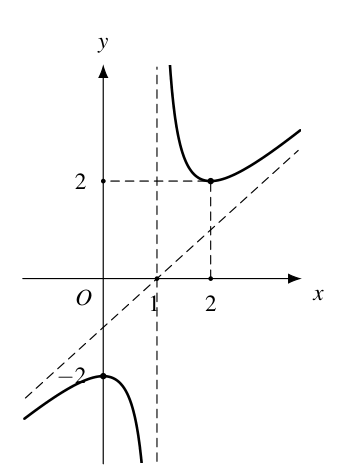
\includegraphics[width=4.0cm]{p2_c4_hinh.png}
	}
	\loigiai{}
\end{ex}

\newpage
\begin{flushleft}
	{\color{blue!50!green}\fbox{\fontfamily{qag}\bfseries\selectfont PHẦN III. Câu trắc nghiệm yêu cầu trả lời ngắn}}
	\textit{\small (Thí sinh trả lời từ câu 1 đến câu 6.)}
\end{flushleft}
\setcounter{ex}{0}
\setcounter{bt}{0}

% Phần III Câu 1
\begin{ex}
	Cho hàm số $y = f(x) = x^3 + 3x^2 - 24x + 1$. Tính tổng các giá trị của $x$ tại đó hàm số đạt cực trị.
	\par\shortans[oly]{-2}
	\loigiai{}
\end{ex}

% Phần III Câu 2
\begin{ex}
	Cho hàm số $y = \dfrac{3x - 2}{x + 1}$. Gọi $I(a; b)$ là giao điểm hai đường tiệm cận. Tính $ab$.
	\par\shortans[oly]{-3}
	\loigiai{}
\end{ex}

% Phần III Câu 3
\begin{ex}
	Cho hàm số $y = f(x)$ có bảng biến thiên như dưới đây:
	\begin{center}
	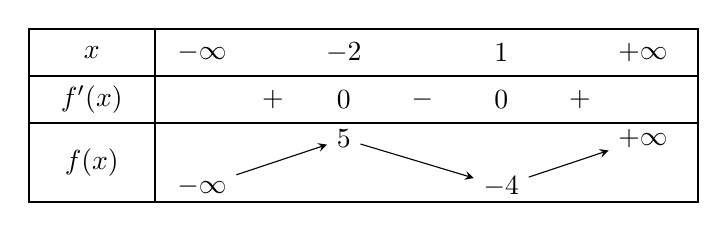
\begin{tikzpicture}[>=stealth,scale=1]
	  \draw[thick] (0,0) rectangle (8.5,-2.2);
	  \draw[thick] (0,-0.6) -- (8.5,-0.6);
	  \draw[thick] (0,-1.2) -- (8.5,-1.2);
	  \draw[thick] (1.6,0) -- (1.6,-2.2);
	  \node at (0.8,-0.3) {$x$};
	  \node at (0.8,-0.9) {$f'(x)$};
	  \node at (0.8,-1.7) {$f(x)$};
	  \node at (2.2,-0.3) {$-\infty$};
	  \node at (4.0,-0.3) {$-2$};
	  \node at (6.0,-0.3) {$1$};
	  \node at (7.8,-0.3) {$+\infty$};
	  \node at (3.1,-0.9) {$+$};
	  \node at (4.0,-0.9) {$0$};
	  \node at (5.0,-0.9) {$-$};
	  \node at (6.0,-0.9) {$0$};
	  \node at (7.0,-0.9) {$+$};
	  \node (p1) at (2.2,-2.0) {$-\infty$};
	  \node (p2) at (4.0,-1.4) {$5$};
	  \node (p3) at (6.0,-2.0) {$-4$};
	  \node (p4) at (7.8,-1.4) {$+\infty$};
	  \draw[->] (p1) -- (p2);
	  \draw[->] (p2) -- (p3);
	  \draw[->] (p3) -- (p4);
	\end{tikzpicture}
	\end{center}
	Tính hiệu giữa giá trị cực đại và giá trị cực tiểu của hàm số.
	\par\shortans[oly]{9}
	\loigiai{}
\end{ex}

% Phần III Câu 4
\begin{ex}
	Cho hàm số $y = \dfrac{x^2 + 2x + 5}{x + 1}$. Tính hoành độ giao điểm của hai đường tiệm cận của đồ thị.
	\par\shortans[oly]{-1}
	\loigiai{}
\end{ex}

% Phần III Câu 5
\begin{ex}
	Cho hàm số $y = f(x)$ có đạo hàm $f'(x) = (x - 2)^2(x + 1)(x - 4)$ với mọi $x \in \mathbb{R}$. Hàm số có bao nhiêu điểm cực trị?
	\par\shortans[oly]{2}
	\loigiai{}
\end{ex}

% Phần III Câu 6
\begin{ex}
	Cho hàm số $y = \dfrac{mx + 3}{2x - 1}$ có tiệm cận ngang $y = 2$. Tính $m$.
	\par\shortans[oly]{4}
	\loigiai{}
\end{ex}

\vspace{0.4cm}
\begin{center}
	\textbf{------ HẾT ------}
\end{center}

\end{document}
